%% This is emulateapj reformatting of the AASTEX sample document
%%
\documentclass[iop]{emulateapj}

%\newcommand{\vdag}{(v)^\dagger}
%\newcommand{\myemail}{skywalker@galaxy.far.far.away}
\usepackage{natbib}
\newcommand{\stsp}{\texttt{STSP}}
\newcommand{\kepler}{\textit{Kepler}}
\usepackage{amsmath}
%% You can insert a short comment on the title page using the command below.

%\slugcomment{To appear in a journal real soon, ya hear?}

%% If you wish, you may supply running head information, although
%% this information may be modified by the editorial offices.
%% The left head contains a list of authors,
%% usually a maximum of three (otherwise use et al.).  The right
%% head is a modified title of up to roughly 44 characters.
%% Running heads will not print in the manuscript style.

\shorttitle{Starspots on HAT-P-11}
\shortauthors{Morris et al.}

%% This is the end of the preamble.  Indicate the beginning of the
%% paper itself with \begin{document}.

\begin{document}

%% LaTeX will automatically break titles if they run longer than
%% one line. However, you may use \\ to force a line break if
%% you desire.

\title{HAT-P-11:\\ A Song of Fire and Magnetism}

%% Use \author, \affil, and the \and command to format
%% author and affiliation information.
%% Note that \email has replaced the old \authoremail command
%% from AASTeX v4.0. You can use \email to mark an email address
%% anywhere in the paper, not just in the front matter.
%% As in the title, use \\ to force line breaks.

\author{Brett M. Morris\altaffilmark{1}}

\author{Leslie Hebb\altaffilmark{2}}

\author{James R. A. Davenport\altaffilmark{3,4}}

\author{Suzanne L. Hawley\altaffilmark{1}}

\email{bmmorris@uw.edu}

%% Notice that each of these authors has alternate affiliations, which
%% are identified by the \altaffilmark after each name.  Specify alternate
%% affiliation information with \altaffiltext, with one command per each
%% affiliation.

\altaffiltext{1}{Astronomy Department, University of Washington,
                 Seattle, WA 98119}
\altaffiltext{2}{Physics Department, Hobart and William Smith Colleges, 
                 Geneva, NY 14456}
\altaffiltext{3}{Department of Physics \& Astronomy, Western Washington University, Bellingham, WA 98225}
\altaffiltext{4}{NSF Astronomy and Astrophysics Postdoctoral Fellow}

%% Mark off your abstract in the ``abstract'' environment. In the manuscript
%% style, abstract will output a Received/Accepted line after the
%% title and affiliation information. No date will appear since the author
%% does not have this information. The dates will be filled in by the
%% editorial office after submission.

\begin{abstract}
We found all of the things.
\end{abstract}

%% Keywords should appear after the \end{abstract} command. The uncommented
%% example has been keyed in ApJ style. See the instructions to authors
%% for the journal to which you are submitting your paper to determine
%% what keyword punctuation is appropriate.

%% Authors who wish to have the most important objects in their paper
%% linked in the electronic edition to a data center may do so in the
%% subject header.  Objects should be in the appropriate "individual"
%% headers (e.g. quasars: individual, stars: individual, etc.) with the
%% additional provision that the total number of headers, including each
%% individual object, not exceed six.  The \objectname{} macro, and its
%% alias \object{}, is used to mark each object.  The macro takes the object
%% name as its primary argument.  This name will appear in the paper
%% and serve as the link's anchor in the electronic edition if the name
%% is recognized by the data centers.  The macro also takes an optional
%% argument in parentheses in cases where the data center identification
%% differs from what is to be printed in the paper.

\keywords{greatness, glory, star-spot-sleuthery}

%% From the front matter, we move on to the body of the paper.
%% In the first two sections, notice the use of the natbib \citep
%% and \citet commands to identify citations.  The citations are
%% tied to the reference list via symbolic KEYs. The KEY corresponds
%% to the KEY in the \bibitem in the reference list below. We have
%% chosen the first three characters of the first author's name plus
%% the last two numeral of the year of publication as our KEY for
%% each reference.

\section{Introduction}

NASA’s Kepler mission measured rotational flux modulations of thousands of stars over its four-year mission. The flux variations are caused by dark starspots moving into and out of view as stars rotate \citep{McQuillan2014}, and these variations encode valuable information about magnetic activity and differential rotation near the photosphere \citep{Davenport2015}. Spot positions can be measured from photometry with photometric inversion \citep{Roettenbacher2013} or by direct spot modeling \citep{Frasca2011}, but the spot position precision is limited due to degeneracies between the stellar obliquity and the spot latitude, longitude, and radius. 

Some of these degeneracies can be broken for host stars of transiting planets, giving us access to precise positions of starspots. The flux lost at any instant during a transit event is proportional to the intensity of the occulted portion of the stellar surface. Occultations of starspots by planets are observed as positive flux anomalies in transit light curves, which are well-resolved in time by Kepler short-cadence photometry. Then if the stellar orientation is known via the Rossiter-McLaughlin effect \citep{Ohta2005, Winn2005}, timing of spot occultations can be transformed into precise positions of starspots \citep{Sanchis-Ojeda2011}.

HAT-P-11 is a K4 dwarf with mass $M_\star = 0.8 M_\odot$ and a planet with period $P \equiv 4.88$ d, mass $M_p=0.08 M_J$, and radius $R_p = 0.4 R_J$ \citep{bakos2010}. The planet has a significant orbital eccentricity of $e \sim 0.2$. Observations of the Rossiter-McLaughlin effect revealed that HAT-P-11b likely orbits over the poles of its host star \citep{Winn2010, Hirano2011, Sanchis-Ojeda2011}. Therefore the transit chord of the planet over the star sweeps a path near one stellar longitude across many latitudes. The stellar rotation period and the orbital period of the planet are commensurate at 6:1, which causes transits to occur over the same five stellar longitudes \citep{Beky2014a}.

Spot crossings in the \kepler\ observations can be used to search for active stellar latitudes. \citet{Sanchis-Ojeda2011, Deming2011} noted that the first few quarters of \kepler observations show spot occultations predominantly at two orbital phases, which they attribute to starspots which are concentrated at active latitudes. \cite{Beky2014b} constructed a spot occultation model which they applied to HAT-P-11, and they estimage spot contrasts and [Distinguish our work from this paper]

Measuring spots on HAT-P-11 with spotrod \citep{Beky2014b}

Transmission spectrum: \citep{Fraine2014}

gyrochronological and isochronal ages: \citep{Maxted2014}

\citep{Huber2010}

\section{Transit of HAT-P-11 \lowercase{b}} \label{sec:transit}

%- We first need to fit for the transit parameters in order to fit for the spot parameters later
%- To find the transit parameters, we need to find transits to fit without spot crossings (hard!)
We must first remove the transit of HAT-P-11b from each light curve to study the residual signal imparted by starspots. It is non-trivial to derive the transit parameters for HAT-P-11 b since nearly all of the transits appear to be affected by starspots to some extent. The most robust measurement of the transit properties would be to fit the light curve simultaneously for the transit and the occulted starspots, but the number of parameters in that fit would be prohibitively large. Therefore, we opt to fit for the transit parameters on a subset of transits with minimal starspot anomalies, and to fix those transit parameters later when we marginalize over the starspot properties.

\begin{figure}
\centering
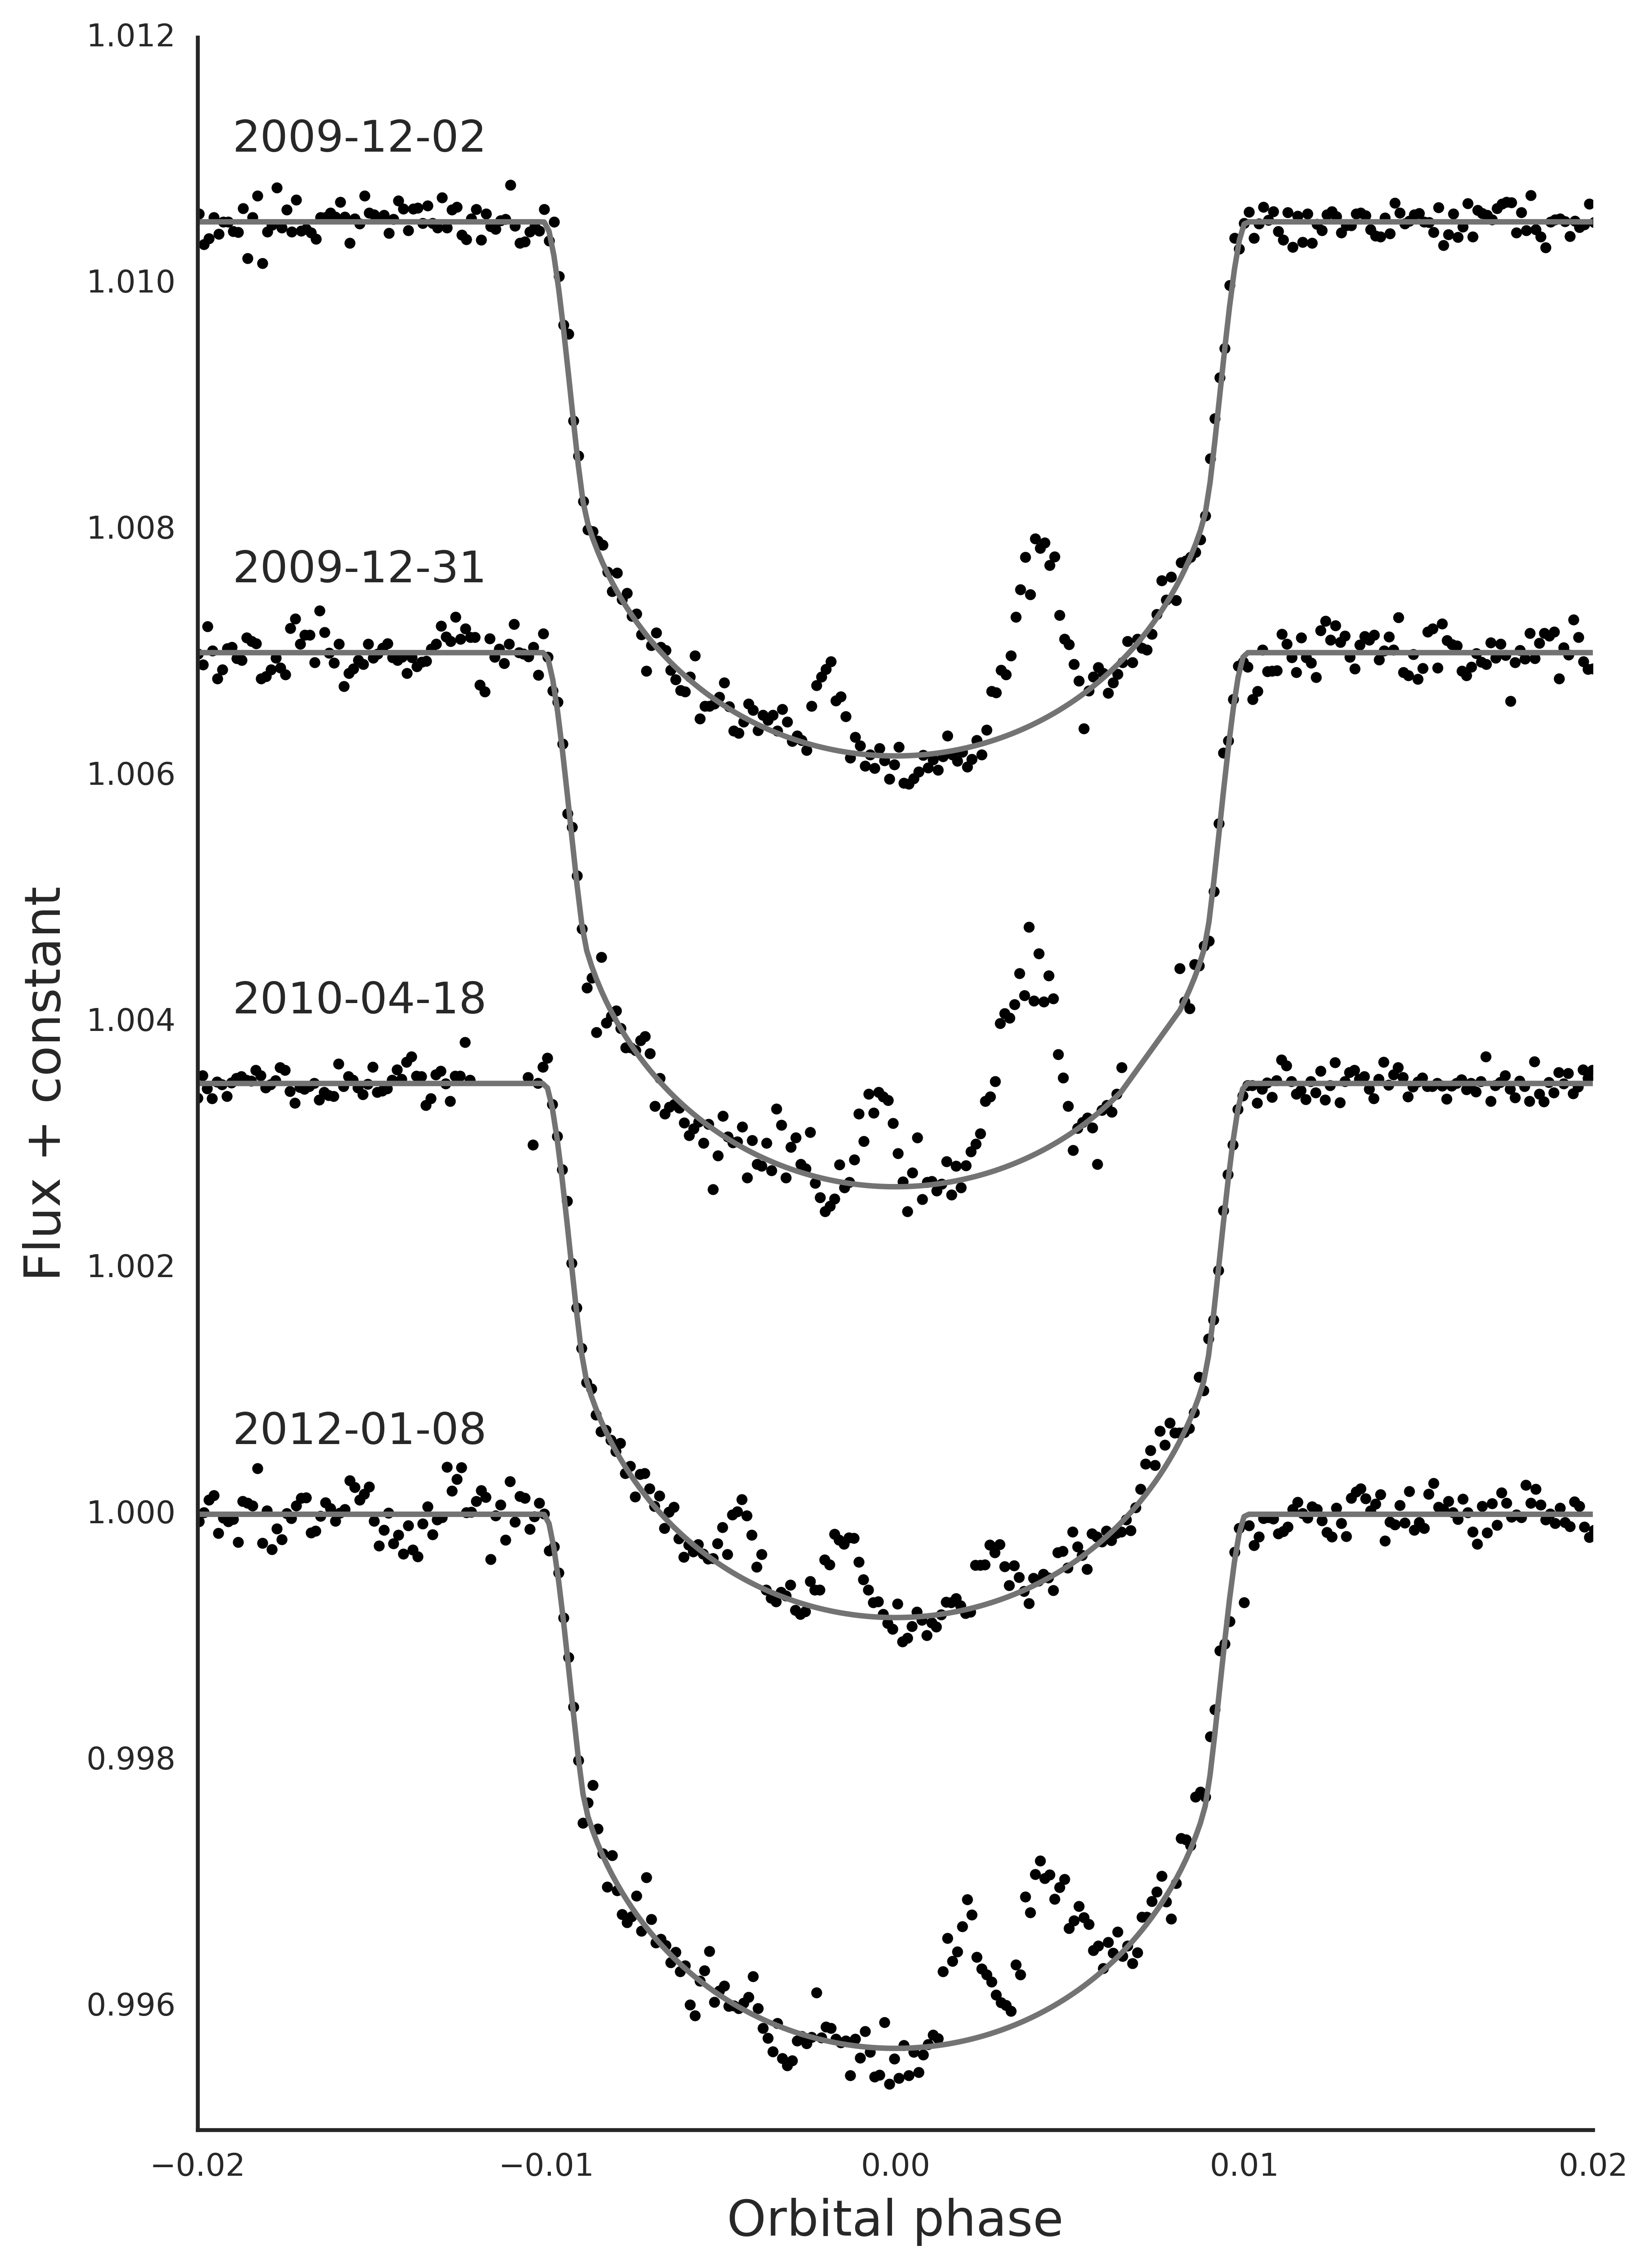
\includegraphics[scale=0.4]{figures/transit_gallery.png}
\caption{Some typical transit light curves of HAT-P-11 b. The points are \kepler\ fluxes, the curves are the best-fit transit model \citep{Mandel2002}. The positive anomalies during transit are occultations of starspots by the planet. }
\label{fig:transit_gallery}
\end{figure}

\subsection{Light Curve Normalization}
%- normalization is important
For the transit depths to be consistent in each transit light curve, an appropriate normalization for each transit must be chosen. Transit light curves are often normalized by the flux immediately before ingress and after egress. Each transit light curve will have different depths if the total flux of the star is varying due to unocculted starspots \citep{Czesla2009, Carter2011, Csizmadia2013}. For example, if unocculted starspots dim the host star's flux by a factor $0 < \epsilon < 1$, the change in flux during transit $\Delta F$ is the same as when the star is not spotted, but the total flux $F$ is smaller, so the depth $\delta = \Delta F / (\epsilon F)$ is larger for the spotted star than for the unspotted star. To avoid the additional computational complexity brought by fitting for the depth in each transit light curve, we normalize the raw \kepler\ transit light curves in a different way, which we call the ``subtract-add-divide'' method. 

%- subtract-add-divide
The baseline flux of the star changes as the star rotates and different starspots are brought into and out of view. If we assume that the peak flux of the star over a few stellar rotations is close to the unobscured brightness of the unspotted star, then we can normalize all transit fluxes by: (1) fitting and subtracting a low-order polynomial to the out-of-transit fluxes near each transit, (2) adding the peak flux to each detrended transit, and (3) dividing each transit by the peak flux. The subtraction by a low-order polynomial removes trends in flux due to stellar rotation, and the addition and division by the peak flux normalizes the out-of-transit fluxes to near-unity, while keeping the transit depths consistent between transits. 

To apply the ``subtract-add-divide'' method to the \kepler\ transit light curves, we first smooth the short-cadence fluxes of each \kepler\ quarter with a Gaussian kernel ($\sigma=700$ cadences) and taking the maximum flux of each quarter. We choose to normalize each quarter with its own independent flux maximum because systematic trends in the \kepler\ photometry change the baseline flux of the star between quarters. We then subtract a second-order polynomial fit to the out-of-transit fluxes near each transit, then add the quarterly peak flux and divide by the quarterly peak flux. 

This normalization method assumes that the peak flux in each quarter is roughly equivalent to the peak flux in every other quarter, which could be a poor assumption if stellar activity on HAT-P-11 varies significantly over timescale of the \kepler\ observations. We will show later that the spot frequency does not appear to vary significantly over the duration of the \kepler\ mission.

%- We find transits without spot crossings with my simple technique
\subsection{``Spotless'' Transits}

We selected ten transits with the fewest measurable starspot crossings to fit for the transit parameters. To identify the transits least perturbed by starspots, we fit a \citet{Mandel2002} transit light curve to each of the 205 normalized short-cadence transits in the Kepler light curve. We hold the light curve parameters fixed except for the depth which is allowed to vary, and optimize the light curve parameters with a Levenburg-Marquardt least-squares minimizer. The light curve fits with the smallest $\chi^2$ are the ones with the fewest spot crossings, since spots cause deviations in the light curve from a normal transit, inflating the $\chi^2$. We then solve for the transit light curve parameters with MCMC, using \texttt{emcee} \citep{Foreman-Mackey2013}. There are no highly significant starspot crossings visible by eye after this selection process, see Figure~\ref{fig:spotlesstransits}. The transit parameters derived from these light curves are described in Table~\ref{tab:transitprops}.

%- The above technique is likely produces a non-gaussian depth distribution, but it is a sufficient approximation 
The fits to the ``spotless'' transit light curves provide a check on the ``subtract-add-divide'' normalization technique and on how spotless those transits really are. If the normalization technique failed to normalize the variation in apparent depth due to unocculted starspots, the transit residuals would be weighted towards more negative fluxes during the transit for transits with more (or darker) unocculted spots. If the ``spotless'' transit identification technique failed, we would expect localized anomalies when starspots were occulted. The scatter in the residuals is larger during transit than out of transit, but only by a factor of XXX, so we conclude that the normalization and ``spotless'' transit identification are sufficient.


\begin{table}
\centering
\begin{tabular}{cc}
Parameter & Measurement\\ \hline
\input{results/hat-11_light_curve_params.txt}
\hline
\end{tabular}
\caption{Transit light curve parameters for HAT-P-11 from the ten transits in Figure~\ref{fig:spotlesstransits}. $T_{14}$ is the duration between first and fourth contact. $q_1$ and $q_2$ are the limb-darkening parameters of \citet{Kipping2013}. These parameters are fixed for the starspot fits. }
\label{tab:transitprops}
\end{table}

\begin{figure}
\centering
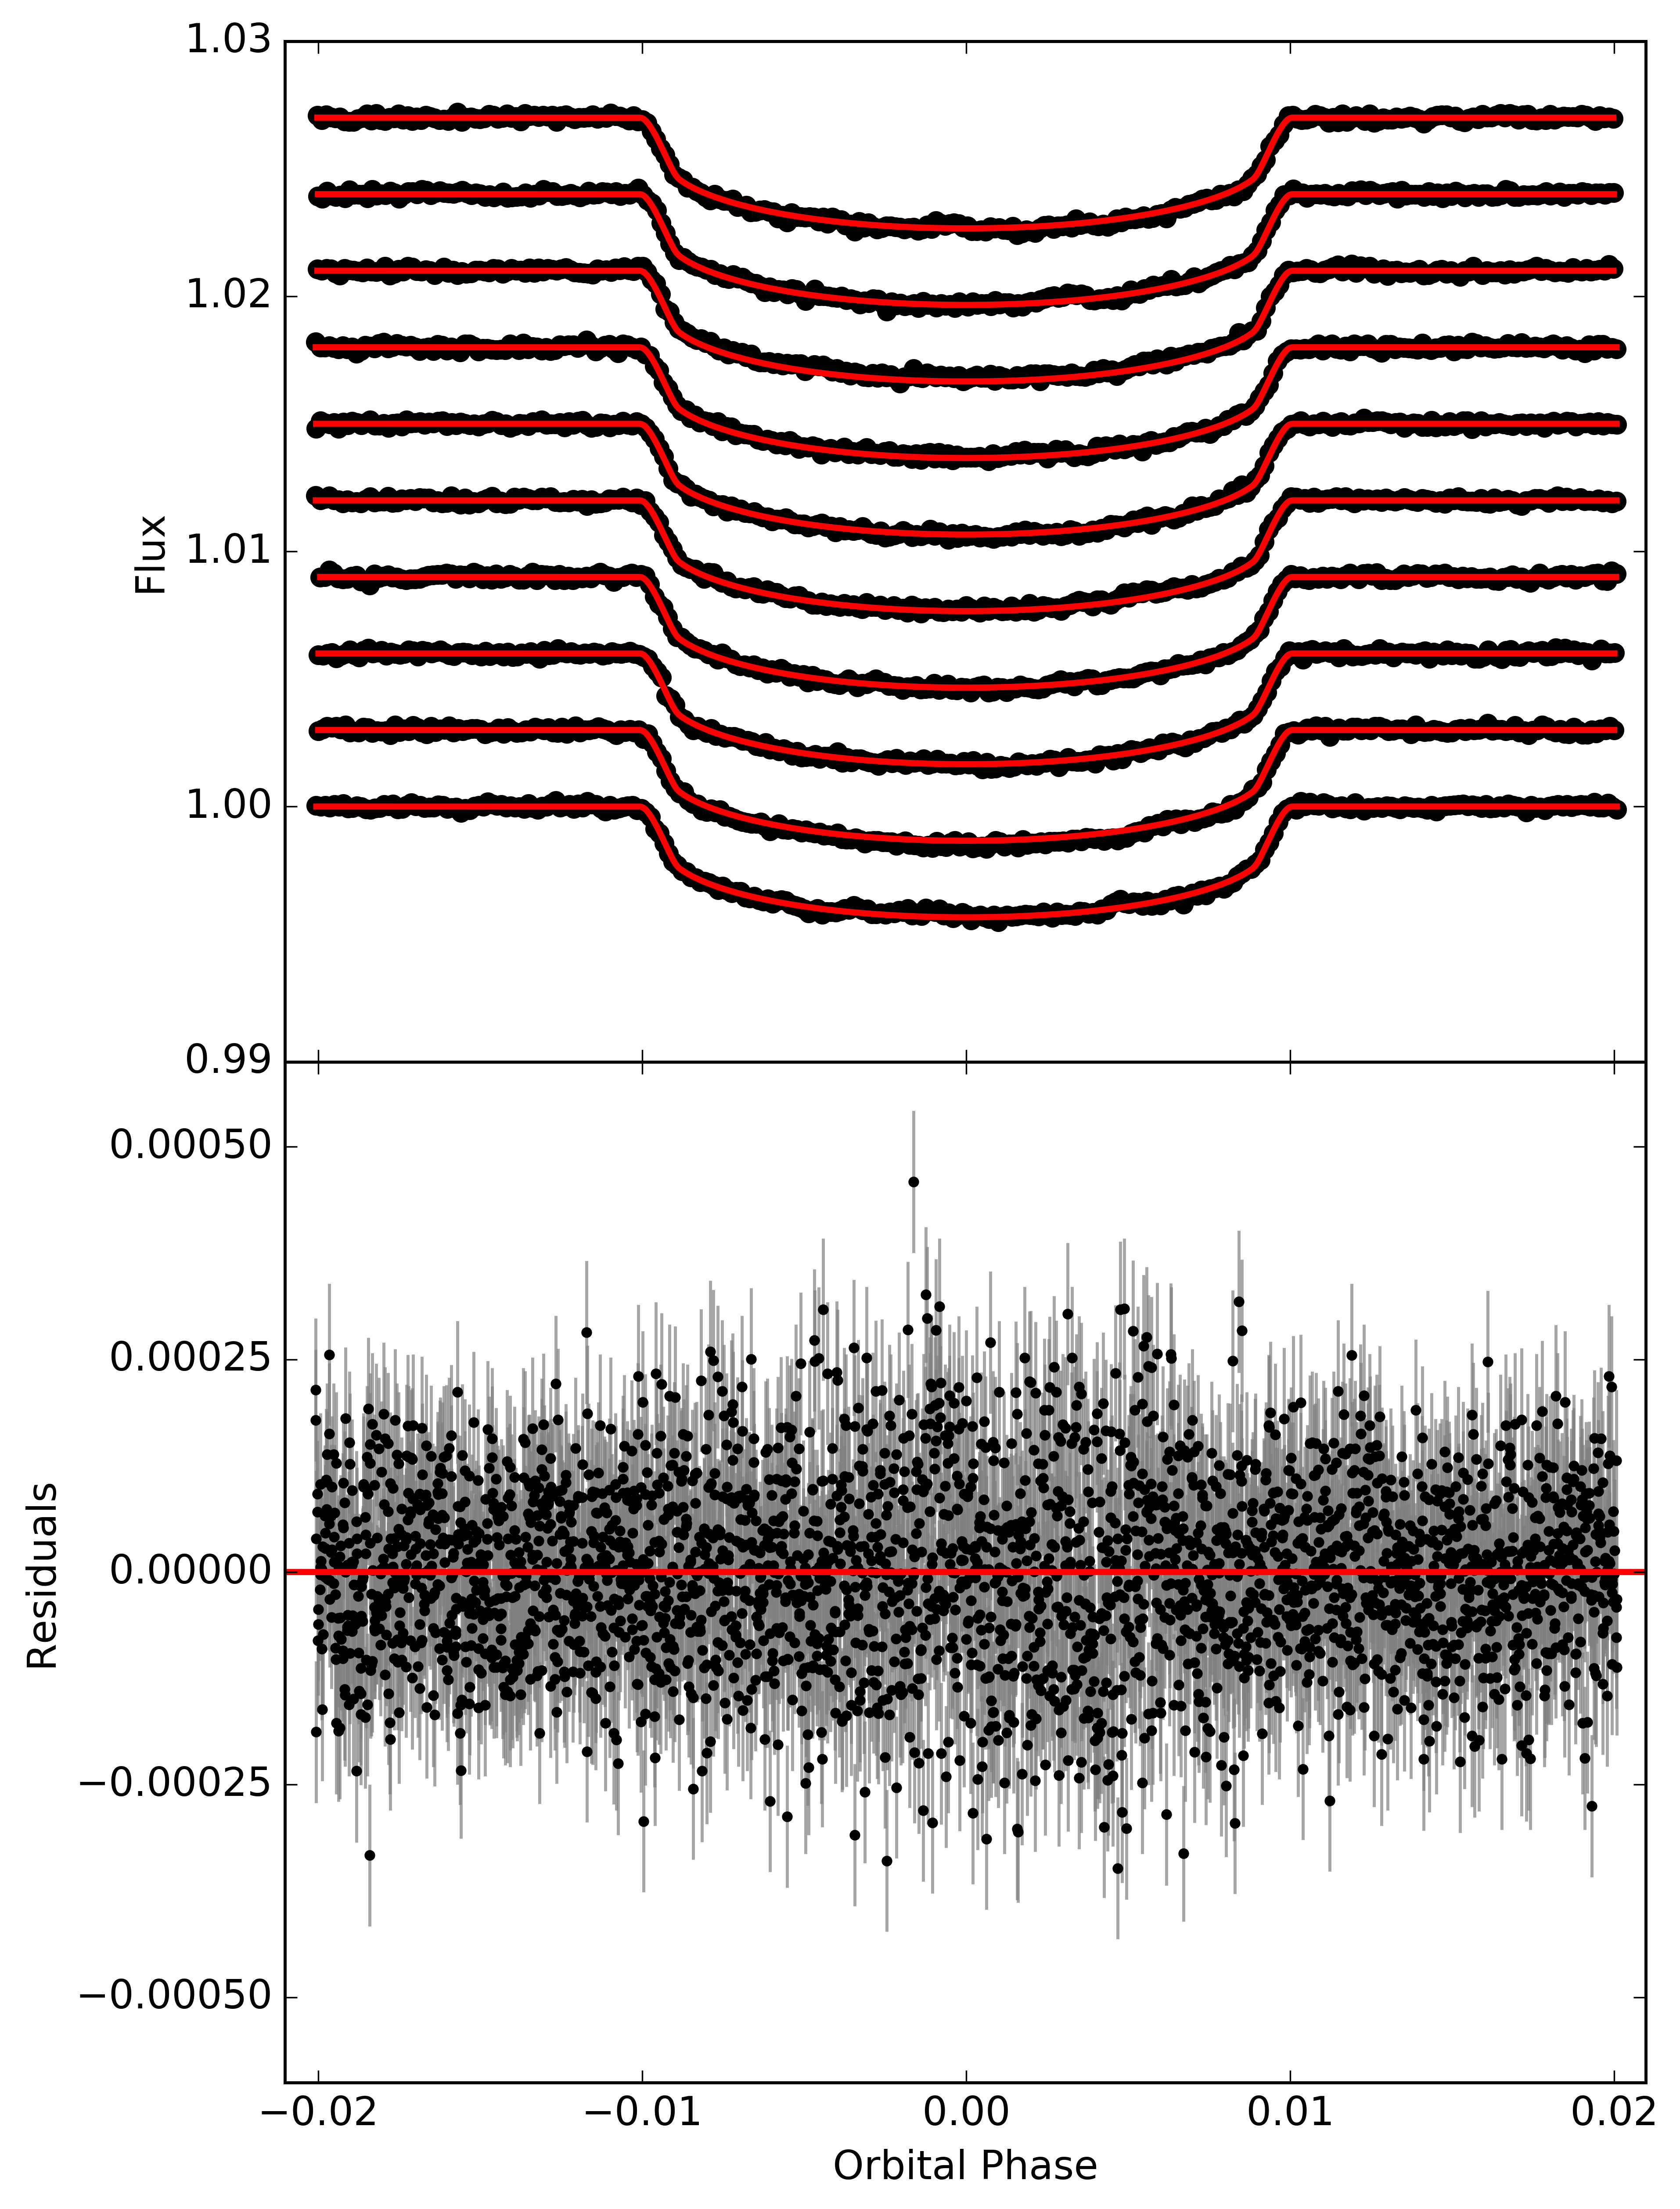
\includegraphics[scale=0.42]{figures/hat11_spotless_transits_compact.png}
\caption{The ten transits least affected by starspot crossings. Transit parameters are listed in Table~\ref{tab:transitprops}.}
\label{fig:spotlesstransits}
\end{figure}

%- We find agreement with these previously published transit parameters, and resolve a tension in the literature for these other ones

The best-fit transit parameters are listed in Table~\ref{tab:transitprops}. Measurements of the mean stellar density of HAT-P-11 via asteroseismology and transit light curves constraints have been reported by \citet{Christensen-Dalsgaard2010} and \citet{Southworth2011}, respectively. Using our transit parameters for HAT-P-11 b, we constrain the mean stellar density $\rho_s = \input{results/stellar_density.txt}$ g cm$^{-3}$, which is significantly smaller than the asteroseismic value of $\rho_s \sim 2.5127$ g cm$^{-3}$ \citet{Christensen-Dalsgaard2010} and significantly less than the photometric value of $\rho_s = 3.40 \pm 0.13$ g cm$^{-3}$ \citet{Southworth2011}.

\section{Spot Occultation Model}

% 2.2 Spot Occultation Model

% - Describe the degeneracies that make locating starspot positions so difficult to retrieve
It is notoriously difficult to measure starspot positions robustly. For example, \citet{Aigrain2015} did a ``blind hare-and-hounds exercise'' in which five teams attempted to deduce stellar rotation periods and differential rotation in an ensemble of model \kepler-like light curves. While most teams could agree on the stellar rotation periods, starspot modeling yielded little agreement on the differential rotation shear. 

% - Refer to the (forthcoming) Davenport paper that demonstrates that model convergence is elusive/expensive for unseeded spot models

One reason for the disagreement is the number of degenerate quantities encoded in the photometry. Photometric variability due to stellar rotation is a function of the stellar rotation period, the stellar obliquity (defined by two angles), the starspot latitudes and longitudes, the differential rotation rate, the spot contrasts and radii, and more. In some special cases, unique solutions to starspot positions are attainable. For example, \citet{Davenport2015} measured the positions of starspots and the differential rotation rate for the M4 dwarf GJ 1243. This light curve was exceptionally ammenable to photometric inversion because it has two dominant spots that impart strong $\sim 3$\% flux variations in the light curve, with spot lifetimes of years. It is much more difficult to measure the starspot positions if each spot is only visible for $\lesssim$one a stellar rotation, as is the case for solar-like stars, without additional means of breaking the position degeneracies.

The degeneracies in starspot positions can be broken for host stars of transiting exoplanets. The shape of the transit light curve defines the transit chord over the surface of the star, and the Rossiter-McLaughlin effect measures the stellar obliquity, thus we can measure the latitudes and longitudes of the stellar surface occulted by a planet throughout a transit event. Then when the planet occults a dark starspot, the timing and shape of the positive flux anomaly in the transit light curve can be transformed into the position of the starspot on the star. 

CITE-LESLIE developed a flux model for spotted stars with transiting planets called \stsp, which leverages spot occultations during planetary transits to break the spot position degeneracies. CITE-JIM solved for the positions of the starspots of the well-aligned system Kepler-17 with \stsp, in which the planet appears to orbit roughly along the stellar equator. The \stsp\ model is therefore able to recover position information from spots near the stellar equator in multiple consecutive transits, which is useful for probing spot evolution at one latitude. 

Unlike Kepler-17, HAT-P-11 b's orbit normal is nearly perpendicular to the host star's spin -- in other words, it nearly orbits over the host star's poles. Therefore each transit cuts a chord across the stellar surface from pole to pole, across most latitudes at roughly one longitude (XXX need a figure to show this). The light curve of HAT-P-11 thus encodes the starspot distribution with latitude, which CITE-DAVENPORT could not probe with Kepler-17.

The starspots of HAT-P-11 are not occulted by the planet in consecutive transits, unlike Kepler-17. Since the stellar rotation period is roughly $P\sim 30$ d and the orbital period is $P \sim 5$ days, the planet occults the same longitude once per stellar rotation, which appears to be longer than the lifetime of spots on HAT-P-11 \citep{Sanchis-Ojeda2011}. We thus can not observe the same spot in consecutive transits, and we would gain few if any additional constraints by simultaneously fitting consecutive transits as CITE-JIM did. 

% - These degeneracies lead us to find better initial spot parameters by optimizing an approximate light curve model first, then using the detailed forward-model of Hebb et al.. We explain both approaches below.
In the absense of multiple occultations of each spot, we take a different approach to optimizing the \stsp\ model for the spot occultations of HAT-P-11. The starspot occultations impart only small anomalies to a few cadences in transit, so the spot model has a very sharply pitted $\chi^2$-surface to explore, which poses a challenge for efficient optimization. CITE-JIM found that the chains required expensive, long convergence times to fully explore the parameter space before settling into local minima in $\chi^2$, which they assumed to be global minima after a certain number of MCMC steps (XXX is this true?). Even though spot occultations of HAT-P-11 do not reoccur in multiple transits, individual spot occultations on HAT-P-11 have higher signal-to-noise than equivalent spot occulations on Kepler-17 because HAT-P-11 ($K_p = 9.17$) is significantly brighter than Kepler-17 ($K_p = 14.14$). Therefore, HAT-P-11 spot occultations yield single, high S/N snapshots of individual spots which probe the distribution of spots with latitude, in comparison to the Kepler-17 spot occultations which probe spot evolution at one latitude.

To avoid running MCMC simulations for extremely long integration times for starspot positions without assurances that they are converging to sensible $\chi^2$-minima, we take a different approach from the unseeded parameter sweeps of XXX-CITE-JIM. We first devise a heuristic spot occultation model in Section~\ref{sec:friedrich}, which provides us with sensible initial conditions for the full \stsp\ forward model, which we discuss in Section~\ref{sec:stsp}.


\subsection{Initial, Heuristic Spot Occultation Model} \label{sec:friedrich}
% 2.2.1 Initial, Heuristic Spot Occultation Model

% - What we model: Describe shapes of spot crossing anomalies, their frequency and duration; motivate Gaussian approximation of spot occultations
We observe starspot occultations as positive flux anomalies during transit events. If the starspot is a uniformly dark circular region on the star, and the planet passes over the edge of the spot in a grazing occultation, the resulting flux anomaly is an inverted ``v'' shape, like an inverted eclipsing binary light curve of stars with similar masses. If the planet completely occults the spot or the spot completely circumscribes the planet, the resulting flux anomaly is an inverted ``u'' shape, like an inverted exoplanet transit event. There are many more partial spot occultations (well approximated by Gaussians) than others. In most \kepler\ transits of HAT-P-11, there are between one and five spot occultations with amplitudes more than a few times the noise.

% - How we model: Describe technique for searching for occultation “peaks” in transit residuals, then fitting peaks with Gaussians
We find spot occultations in the transits in a two-step process. First, we subtract the light curve by the transit model from Section~\ref{sec:transit}, which produces residuals near zero except near spot occultations. We then smooth the flux residuals by convolving them with a Gaussian kernel, and apply a local-maximum peak-finding algorithm to find the times and amplitudes of positive anomalies in the residuals. We exclude any peaks detected within 5\% of one transit duration from ingress or egress. Spots occulted near transit ingress and egress are located near to the stellar limb, and we are unlikely to measure reliable spot properties for these highly foreshortened spots. With these candidate spot occultations identified, we can now measure the approximate spot occultation properties, which we will become inputs to the detailed \stsp\ model.

We approximate spot occultations as Gaussians perturbations to the transit light curve residuals. For a transit with $N$ spots, we fit a model to the flux residuals which consists of the sum of $N$ Gaussians. We marginalize over the Gaussian amplitude, mid-occultation time and width parameters using the affine-invariant Markov Chain Monte Carlo pacakge \texttt{emcee} \citep{Foreman-Mackey2013}. We assign a positive prior to the amplitude to search only for occultations of dark spots. We apply a flat logarithmic prior to the mid-spot occultation time to exclude spots occulted within 5\% of the transit duration from transit ingress or egress. We apply a flat logarithmic prior to the spot-occultation width $\sigma$ such that $1.5 < \sigma < 8.6$ minutes. The lower limit on $\sigma$ prevents the model from choosing very narrow Gaussians that affect single fluxes, which are susceptible to outliers. The upper limit on $\sigma$ prevents the model from choosing very broad Gaussians, which we do not observe in the \kepler\ data.
% - How well we model Part 1: Describe possible shortcomings of this approximation, and why we think those are OK approximations


% - How well we model Part 2: Describe quality of algorithm via results of the null test (searched for spots where there are none, no false positives were found).
We run a null test to verify that false-positives are unlikely in this hueristic spot-finding scheme. We offset the mid-transit time by one quarter of an orbital phase and set $R_p/R_\star = 0$ to search for false-postive spot-occultations, in regions of the light curve where no transit is occurring. If there was significant correlated noise in the HAT-P-11 light curve with amplitudes and time-scales similar to the spot-occultation signals, it would be detected as a candidate spot occultation in this run. No such false spot-occultations were detected by the peak-finding algorithm. We therefore conclude that correlated noise is not likely to produce false-positive detections of spot occultations.

% - What to do with model Part 1: 

% - What to do with model Part 2: Describe how these Gaussian occultation fits are converted to stellar lat/lon, to be used as inputs for the detailed STSP model

\subsubsection{Stellar Inclination}

% stellar orientation defined by two angles, lambda from RM, i-s from being clever somehow

The starspot positions that we extract are only as reliable as the stellar orientation that we assume when computing the spot positions. Two angles define the orientation of the stellar rotation axis: (1) the stellar inclination $i_s$, which is the angle between the observer, the center of the star, and the rotational pole of the star; and (2) the projected spin-orbit angle $\lambda$, which is the tilt of the stellar rotational pole on the sky-plane with respect to the orbit normal of the planet (see Figure 1 of \citealt{Fabrycky2009} for a graphical representation of the angles). 

% you can estimate i_s by assuming symmetric active latitudes

The projected spin-orbit angle $\lambda$ can be constrained with the Rossiter-McLaughlin effect, but the stellar inclination $i_s$ is more difficult to measure. The stellar inclination can be calculated for systems with known stellar rotation periods and projected rotational velocity ($v \sin i_s$) measurements, but \citet{bakos2010} found only weak constraints on the projected rotational velocity. In the absence of robust estimates of $i_s$, \citet{Sanchis-Ojeda2011} noted that the distribution of starspots on HAT-P-11 resembled active latitudes like those of the Sun. They required the active latitudes to be symmetric across the stellar equator, which allowed them to fit for $i_s$. \citet{Sanchis-Ojeda2011} measured the positions of the active latitudes and thus $i_s$ with observations from \kepler\ Quarters 0-2, and thus of the complete \kepler\ light curve may yield a stronger constraint on the positions of the active latitudes.

% We do that ^^^ 

We fit a probablistic model for the distribution of the spot latitudes to the spot positions from the initial spot model described above. The model 




\subsection{Detailed \stsp\ Spot Occultation Model} \label{sec:stsp}
% 2.2.2 Detailed “STSP” Spot Occultation Model


With the approximate starspot positions derived from the Gaussian fits to spot occultations in Section~\ref{sec:friedrich}, we explore the spot property parameter space with the \stsp\ forward model (CITE LESLIE). \stsp\ is a pure \texttt{C} code for calculating the variations in flux of a star due to spots, both in- and out-of-transit. In this work we consider the spots which can be detected primarily with the spot occultations during transit, since the spot occultations yield tighter constraints on the spot properties than the out-of-transit flux variations.

% - Describe the STSP spot occultation model (parameters, assumptions, advantages)
The \stsp\ model is constructed as follows. The star is represented by a series of discrete concentric circles with intensities decreasing radially outward to approximate limb darkening. Spots on the star are represented as non-overlapping circles that are darker than the local photosphere, which follow the stellar surface in fixed-body rotation. Each spot is defined by four parameters: radius, latitude, longitude, and intensity contrast relative to the photosphere. The planet is represented by an opaque circle, and the relative flux received by the observer is calculated throughout the orbit of the planet. We marginalize over the spot parameters for a user-specified number of spots with  affine-invariant Markov Chain Monte Carlo (MCMC) \citep{Goodman2010}.

% - Describe previous work with STSP (forthcoming Hebb paper, forthcoming Davenport paper)
Leslie and Jim have done cool things with \stsp. Here's a paragraph about them.

% - Describe how we use the heuristic model outputs as STSP inputs to seed MCMC chains


% - Describe distributed computing strategy for efficient model computation despite large number of free parameters

% - Describe convergence tests (hmm I guess we’ll need some convincing ones, won’t we)

% - Describe model outputs and what we’ll do with them in the next section



\section{Results}

\subsection{Latitude Distribution}

\begin{figure*}
\centering
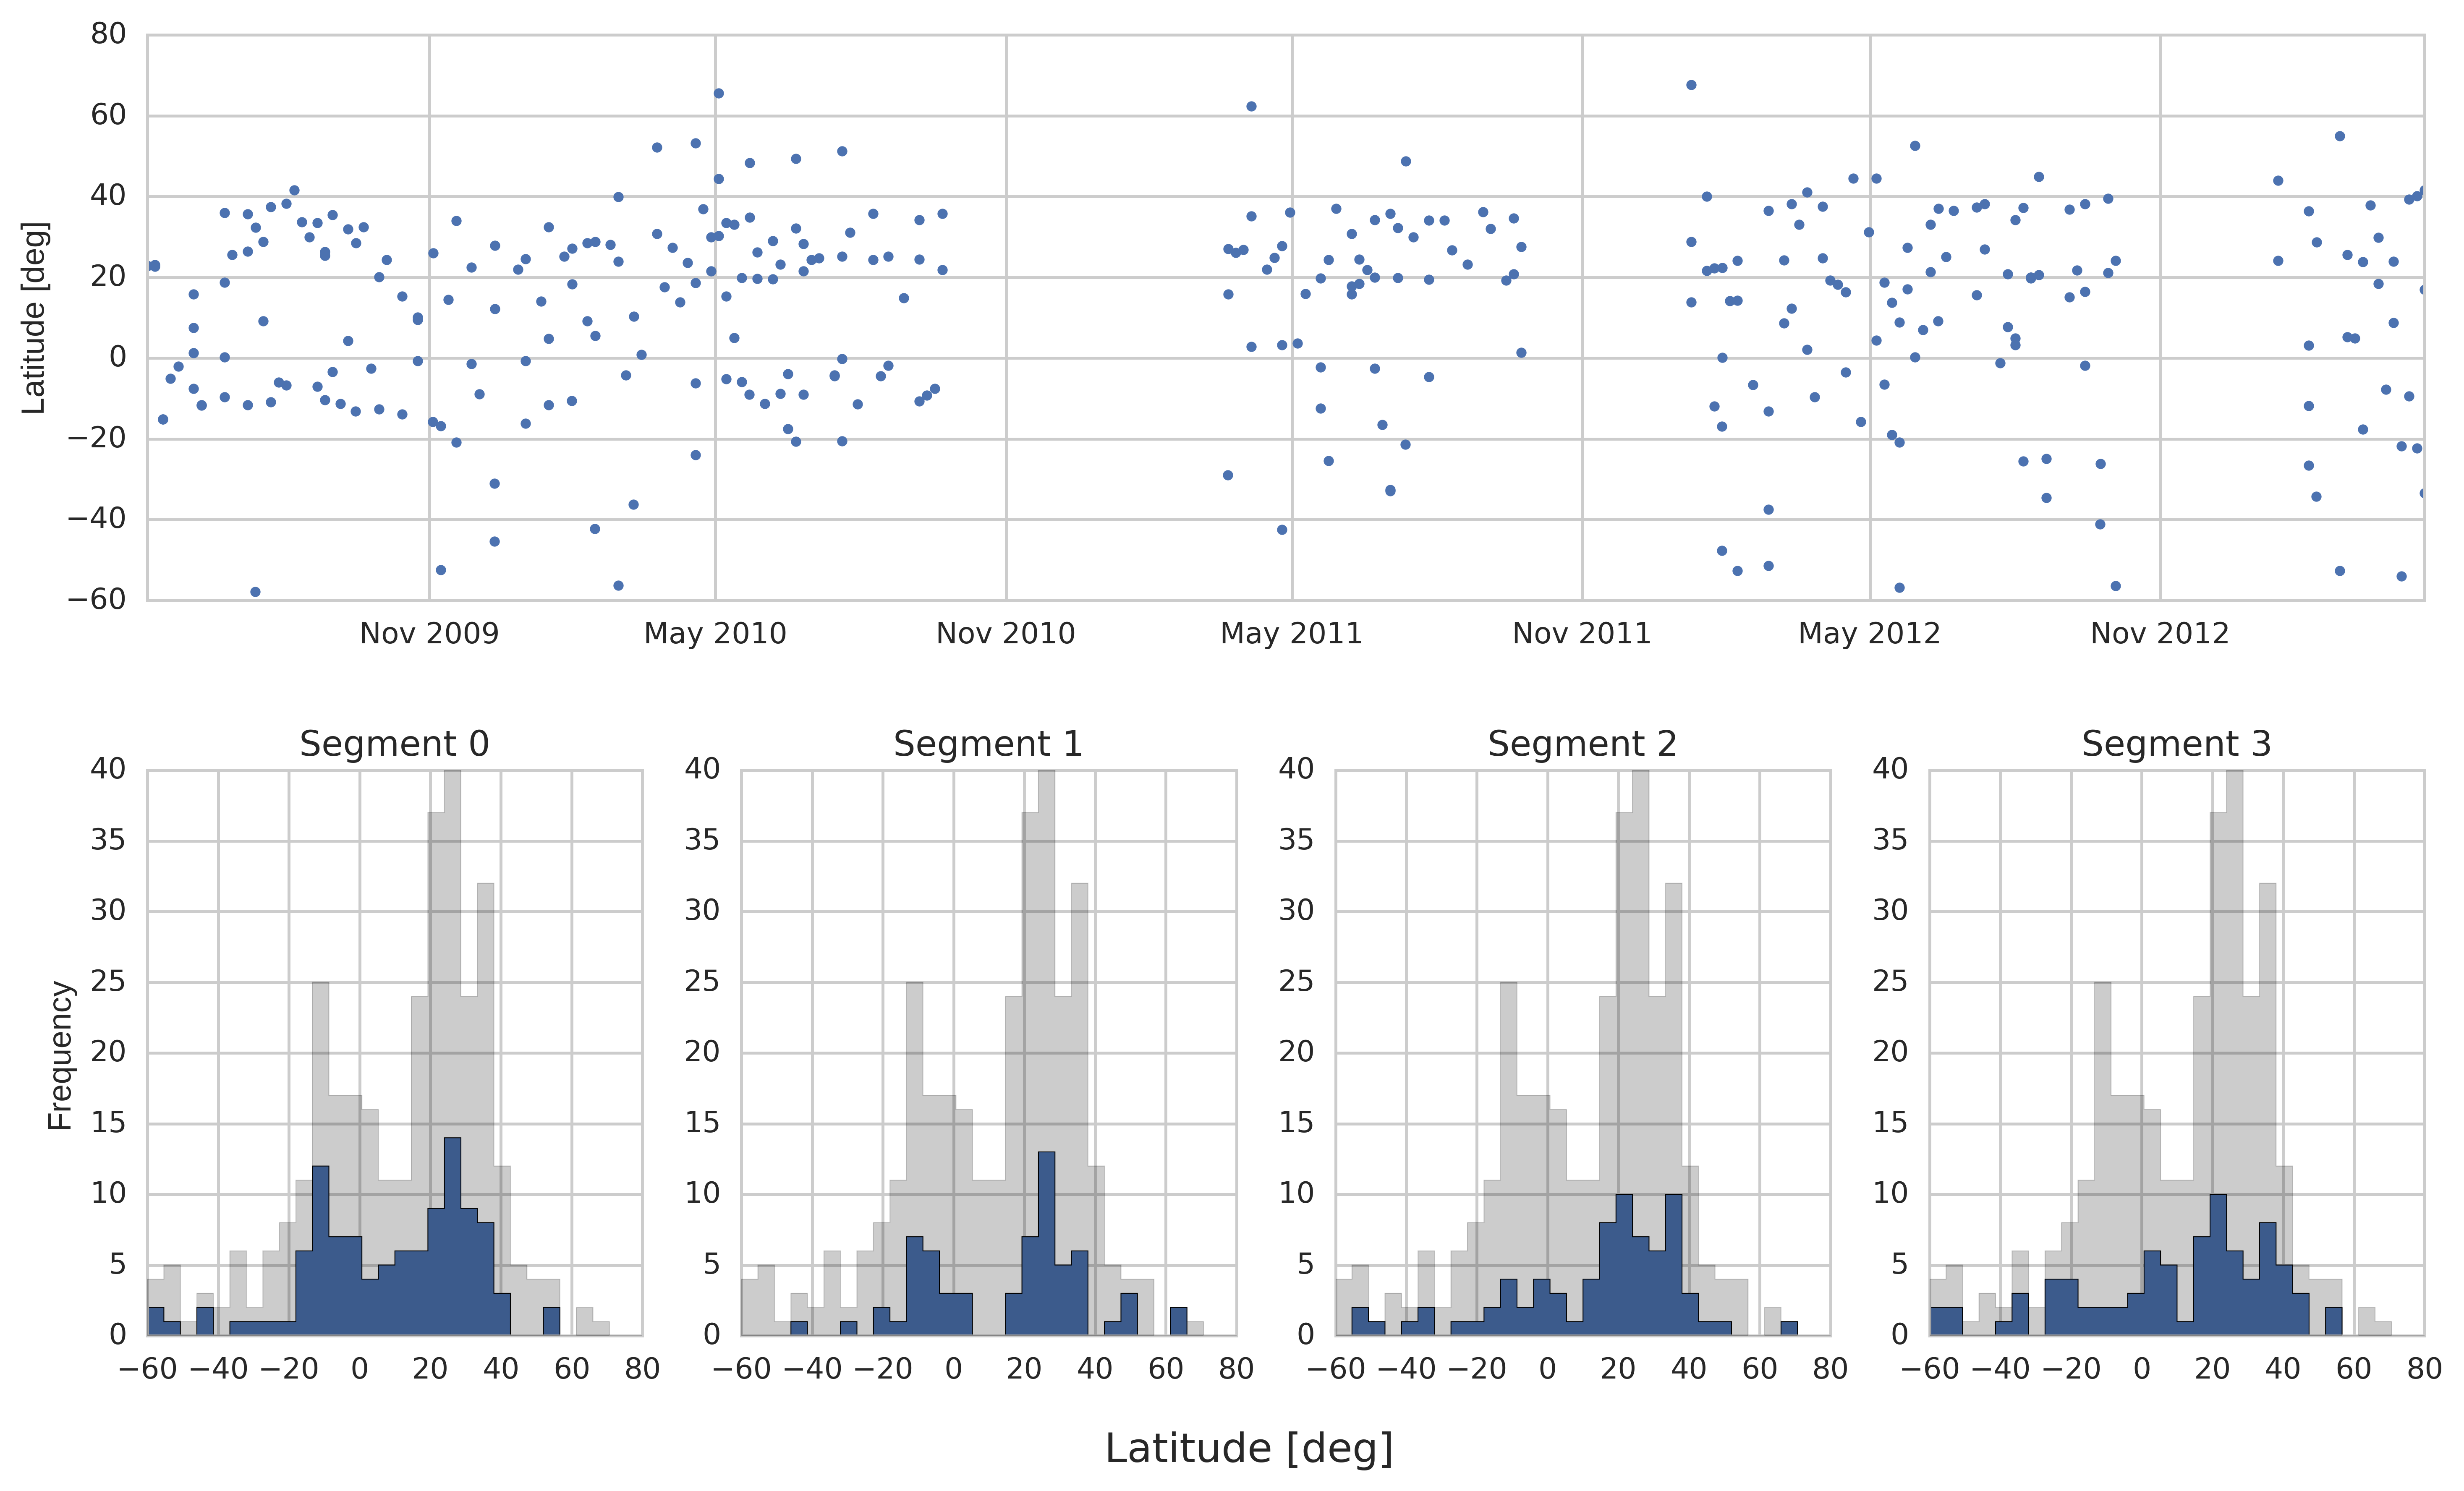
\includegraphics[scale=0.6]{figures/latitude_distribution.png}
\caption{The distribution of spot latitudes may vary with time. \textit{Upper plot}: latitudes of spots recovered with the \stsp\ model. \textit{Lower plots}: the lightly-shaded histograms are the cumulative spot distribution throughout all of the \kepler\ observations. The darker histograms show the frequency distribution of spots within segments of the complete observations, each encompassing one-fourth of the duration of the \kepler\ mission.}
\label{fig:transit_gallery}
\end{figure*}

\subsection{Spot-occultation amplitudes and spot contrasts} \label{sec:contrast}

% Spot contrast is related to the magnetic field strenght. Typical values for sun 
We can compare spot contrasts for spots of HAT-P-11 with sunspots. Typical sunspots have lower temperatures than the local photosphere by roughly $\sim$850 K in the umbra and $\sim$200 K in the penumbra \citep{Eker2003}. In photometric observations we measure the spot intensity contrast relative to the local photosphere $c$ which we define as 
\begin{equation}
c = 1 - I_{sp}/I_{phot}
\end{equation}
where $I_{sp}$ is the intensity inside the dark spot, $I_{phot}$ the intensity of the local photosphere, and $I_{sp} < I_{phot}$. Spots with temperatures and intensities similar to the local photosphere $I_{sp} \equiv I_{phot}$ are ``low contrast'', i.e. $c \rightarrow 0$, and spots with extreme temperature differences $I_{phot} \gg I_{sp}$ are ``high contrast'' and $c\rightarrow 1$. The above umbral and penumbral temperature differences correspond to intensity contrasts of 0.49 and 0.86 (XXX correct these?) respectively in the Kepler bandpass. Solar observations show that regions within spots with higher contrasts correlate with greater magnetic field strength in the vertical component \citep{Keppens1996, Leonard2008}.

% spot occultation amplitude depends on spot size and contrast, so we can measure contrast from amplitude
Spot contrasts can be constrained by the amplitudes of spot occultations events. The difference in flux during a transit with a spot occultation and a transit without a spot occultation is set by the spot contrast and the projected size of the spot compared to the planet. To interpret spot contrasts from the Kepler observations, we derive the amplitude of a spot occultation as a function of the radii of the planet and spot, and the spot contrast. 

We make some simplifying assumptions to derive the spot contrast constraints, and we generalize the formalism later. We will at first calculate the flux only for spot-planet orientations where the planet completely occults the spot or the spot completely encompasses the planet. By ignoring grazing spot occultations, we will calculate maximum spot-occultation amplitudes, since grazing spot occultations yield smaller amplitudes than complete occultations. We also ignore stellar limb darkening.

The flux lost during the transit of a planet with radius $R_p$ across an unspotted star with radius $R_\star$ without limb darkening is
\begin{eqnarray}
\delta_{unspotted} = \frac{\Delta F}{F_\star} = \frac{I_\star \pi R_p^2}{I_\star \pi R_\star^2} = \frac{R_p^2}{R_\star^2}
\end{eqnarray}
where $I_\star$ is the mean surface intensity of the stellar disk per unit area. 

We measure the amplitude of brightening during a spot occultation $A$, see Figure~\ref{fig:contrast_schematic} for a schematic representation. During an occultation of a starspot, the appropriate formula for the observed flux depends on the size of the spot $R_{sp}$ relative to the size of the planet $R_{p}$. If the spot with radius larger than or equal to the radius of the planet $R_{sp} \ge R_p$ and the spot has contrast $c$, the amplitude of the difference in flux between a transit of an unspotted and a spotted star is
\begin{eqnarray}
 A &=& \left. \delta_{unspotted} - \delta_{spotted} \right|_{R_{sp} > R_p} \\
 &=& \frac{I_\star \pi R_p^2}{I_\star \pi R_\star^2} - \frac{((1 - c)I_\star) \pi R_p^2}{ I_\star \pi R_\star^2}\\
 &=& \delta_{unspotted} c. \label{eqn:bigspot}
\end{eqnarray}
For a spot smaller than the planet, the difference between the spotted and unspotted flux is
\begin{eqnarray}
 A &=& \left. \delta_{unspotted} - \delta_{spotted} \right|_{R_{sp} < R_p} \\
 &=& \frac{I_\star \pi R_p^2}{I_\star \pi R_\star^2} - \frac{(c I_\star) \pi R_{sp}^2}{ I_\star \pi R_p^2}\\
 &=& \delta_{unspotted} \left[1-\left(1-c\frac{R_{sp}^2}{R_p^2}\right)\right]. \label{eqn:littlespot}
\end{eqnarray}

% Do we need the below snippet?
In the small planet limit where $R_p/R_\star \ll 1$, the stellar limb darkening could be defined, for example, with a quadratic law $I(\mu)/I_0 = 1 - u_1(1-\mu) - u_2(1-\mu)^2$, and the instantaneous unspotted depth becomes 
\begin{equation}
\delta_{unspotted}(\mu) =  \frac{R_p^2}{R_s^2} \left[ \frac{1 - u_1(1-\mu) - u_2(1-\mu)^2}{1 - \frac{1}{3}u_1 - \frac{1}{6}u_2} \right].
\end{equation}
Equations \ref{eqn:bigspot} and \ref{eqn:littlespot} above can be generalized for stars with limb-darkening by replacing $\delta_{unspotted} \rightarrow \delta_{unspotted}(\mu)$.

In Figure~\ref{fig:contrast} we compare the spot occultation amplitudes $A$ normalized by the flux of an unspotted star at that time during the transit $\delta_{unspotted}$ for a variety of spot contrasts and spot sizes with the observed normalized spot amplitudes. As the spot contrast $c$ increases and the spot becomes darker, the amplitude of the spot occultation increases for spots of any radius. For spots larger than the planet, the contrast controls the maximum occultation amplitude. Therefore the maximum observed spot-occultation amplitude sets an lower bound for the maximum spot contrast. The spot occultation with the largest observed amplitude $A/\delta_{unspotted} \sim 0.49$ requires a spot contrast of $c_{min} \le 0.50$, which is similar to the contrast of in the umbra of a sunspot (as discussed earlier in this section). More typically, the median spot ampltiude $A/\delta_{unspotted} = 0.07$ sets a weak upper limit on the contrast of $c_{median} \le 0.92$. 

% Compare with Beky 2014b


% Note that this is only true if the flux of the star is not changing with time, as described by XXX and XXX

%%%%%%%%%%%%%%%%%%%%%%%%%%%%%%%%%%%%%%%%%%%%%%%%%
%%% First draft of occultation amplitude bit: 

% The maximum flux during a spot occultation is set by the spot size $R_{spot}$, and the spot contrast $c$ (setting aside limb darkening). The spot contrast varies from $c=0$ for a spot with zero temperature, to $c=1$ for a spot with the same effective temperature as the photosphere. Spot contrast is difficult to measure from photometry alone due to the degeneracies with spot size and position, as discussed earlier in Section XXX. However, the amplitude of brightening during a spot occultation gives us a constraint on the spot contrast.

% To interpret spot contrasts from the Kepler observations, we derive the amplitude of a spot occultation as a function of the radii of the planet and spot, and the spot contrast. To simplify the calculation, we will calculate the flux only for spot-planet orientations where the planet completely occults the spot, or the spot completely encompasses the planet. As a result, we will calculate maximum spot-occultation amplitudes, and grazing spot occultations will yield smaller amplitudes.

% For a star with flux $F_\star$ and quadratic limb-darkening parameters $u_1$ and $u_2$, the transit depth without spots $\delta$ is the ratio of the sky-projected areas of the planet, with radius $R_p$, and star with radius $R_\star$,
% \begin{eqnarray}
% \delta(\mu) &=& \frac{\pi R_p^2 F_\star (1 - u_1(1-\mu) - u_2(1-\mu)^2)}{\pi R_\star^2 F_\star (1 - \frac{1}{3}u_1 - \frac{1}{6}u_2) } \\
% &=& \left(\frac{R_p}{R_\star}\right)^2 \frac{1 - u_1(1-\mu) - u_2(1-\mu)^2}{1 - \frac{1}{3}u_1 - \frac{1}{6}u_2}
% \end{eqnarray}
% where $\mu$ is the sky-projected distance of the planet. At the time of the minimum flux, $\mu = \sqrt{1-b^2}$. The depth of the transit during the occultation of a starspot is shallower than an equivalent transit without starspots, and we can calculate the depth during a spot occultation in one of two ways, depending on the size of the planet. 

% If $R_{spot} < R_p$, the depth of the transit during the spot occultaton $\alpha$ is the difference between the flux lost during a transit without a spot and a transit with a spot: 
% \begin{eqnarray}
% \frac{\alpha}{\delta} &=& \frac{F_\star \pi R_p^2 - F_\star(1-c) \pi R_{spot}^2}{F_\star (\pi R_p^2)} \\
% &=& 1 - (1-c)\left(\frac{R_{spot}}{R_p}\right)^2.
% \end{eqnarray}

% If $R_{spot} \ge R_p$, the depth of the transit during a spot occultation depends only on the contrast of the spot,
% \begin{eqnarray}
% \frac{\alpha}{\delta} = \frac{cF_\star (\pi R_p^2)}{F_\star(\pi R_p^2)} = c.
% \end{eqnarray}
% We transform the depth during the occultation $\alpha$ to the amplitude of the spot occultation $A$, measured from the unocculted-transit model flux up to the peak flux during the occultation, $A = \delta(1 - \alpha)$.

% Figure~\ref{fig:contrast} shows the maximum spot occultation amplitudes relative to the unspotted transit depth for a few spot contrasts. As the spot contrast increases and the spot becomes darker, the amplitude of the spot occultation increases for spots of any radius. For spots larger than the planet, the contrast controls the maximum occultation amplitude. Therefore the maximum observed spot-occultation amplitude sets an upper bound for the spot contrast.

% The spot occultation with the largest observed amplitude $A/\delta \sim 0.61$ requires a spot contrast of $c \le 0.38$, which is a significantly greater disparity between the temperatures of the spot and photosphere than is typically observed on the Sun, $c \sim 0.7$. More typically, the median spot ampltiude $A = 0.08$ requires a contrast of at most $c \le 0.91$. 
%%%%%%%%%%%%%%%%%%%%%%%%%%%%%%%%%%%%%%%%%%

\begin{figure}
\centering
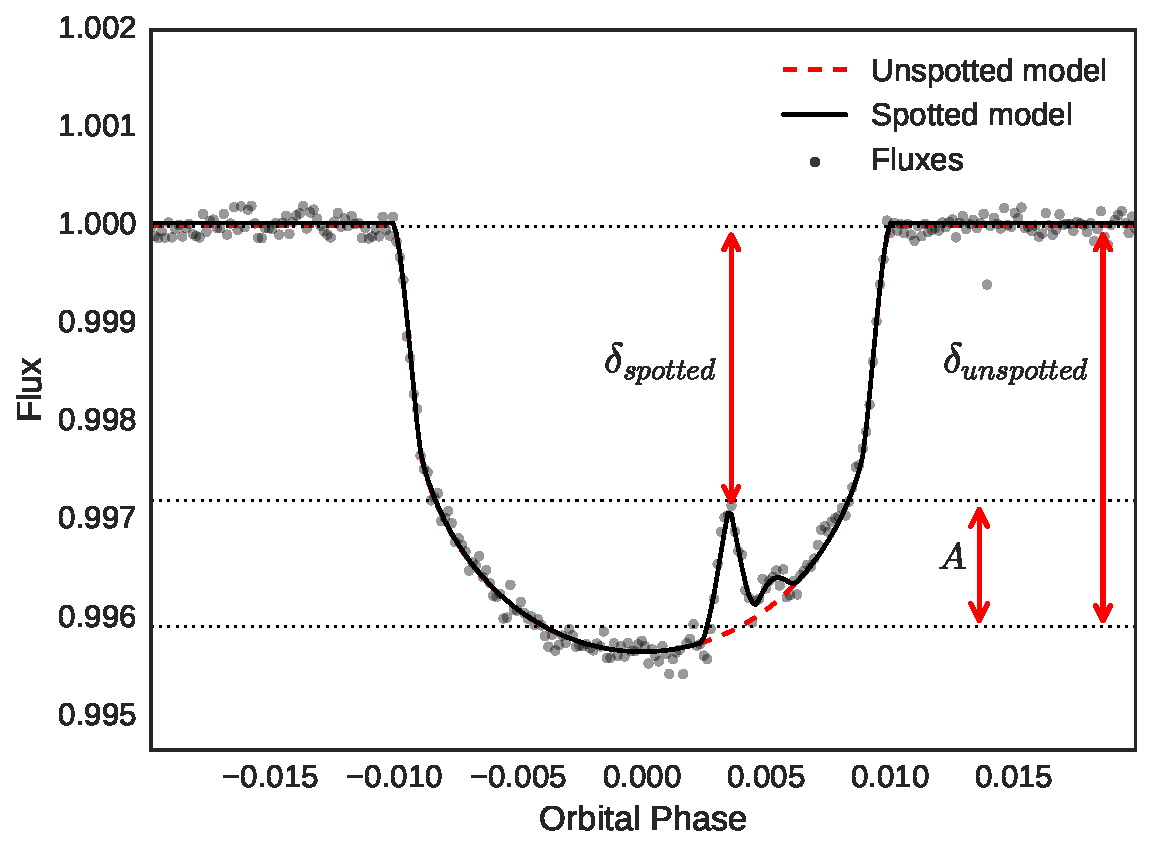
\includegraphics[scale=0.4]{figures/contrast_schematic.pdf}
\caption{Schematic for parameter definitions in Section~\ref{sec:contrast}, plotted on the transit of HAT-P-11 b on August 20, 2011 UT. The spot occultation amplitude $A$ is the difference between the flux lost during a transit with no spot occultations and the flux lost during a transit with spot occultations, $A = \delta_{unspotted} - \delta_{spotted}$. Note that in this terminology the ``depth'' $\delta(\mu) = \Delta F(\mu)/F$ is a function of the sky-projected distance between the planet and the star $\mu$, or equivalently time or orbital phase, for a star with limb-darkening.}
\label{fig:contrast_schematic}
\end{figure}

\begin{figure}
\centering
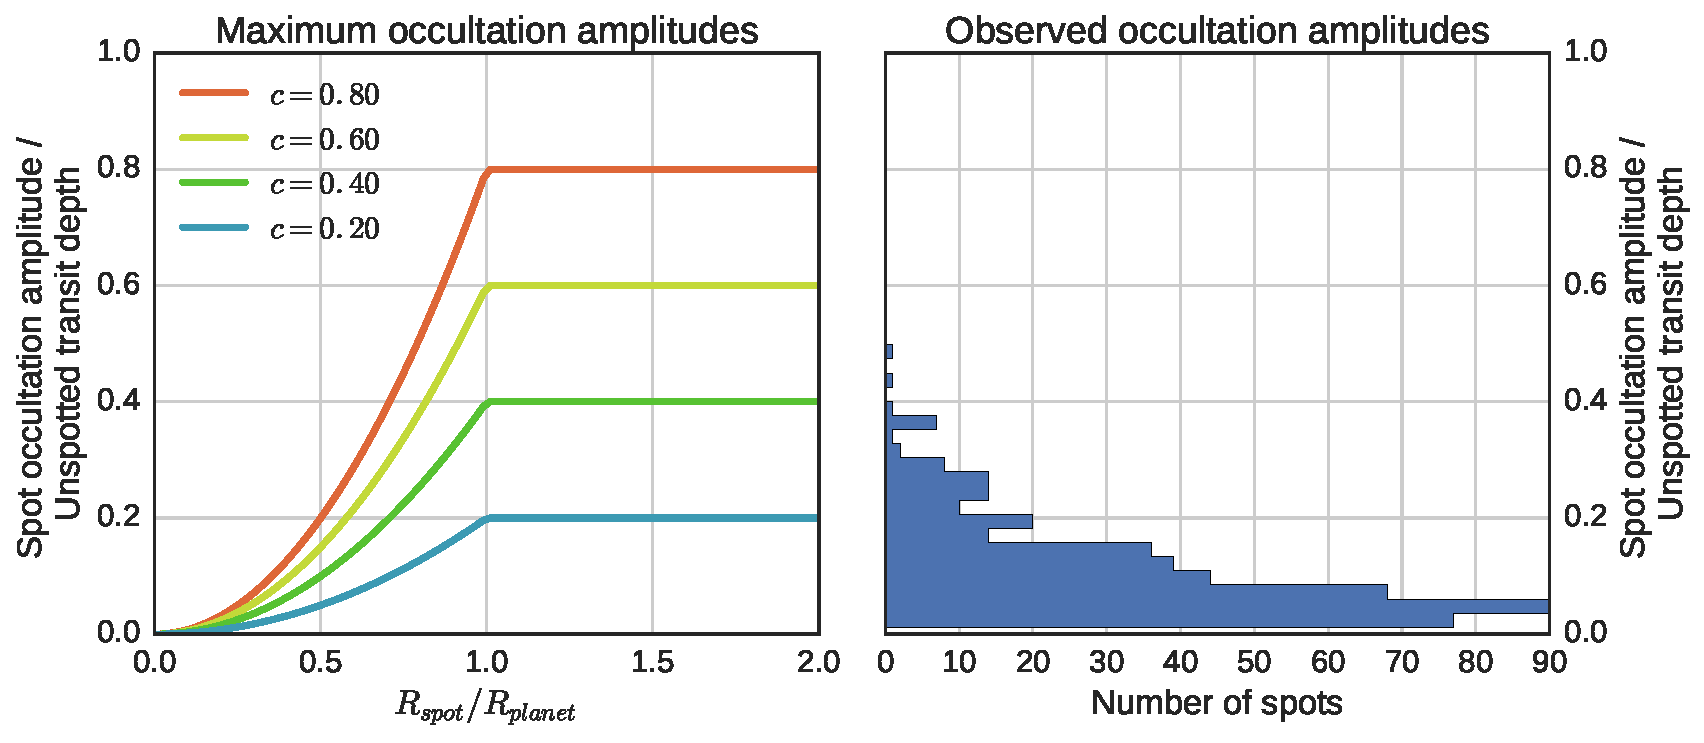
\includegraphics[scale=0.3]{figures/contrasts.pdf}
\caption{\textit{Left:} amplitudes of positive flux anomalies during spot occultations, normalized to the unspotted transit depth, as a function of the spot size and contrast. \textit{Right:} observed spot occultation amplitudes of HAT-P-11. The largest observed spot-occultation amplitude requires a spot contrast $c \le 0.5$, which is a similar to the contrast of sunspot umbra typically observed on the Sun.}
\label{fig:contrast}
\end{figure}


\section{Discussion}

Distribution of spots on cool stars \citep{Schuessler1996, Granzer2000}

\section{Conclusion}


\acknowledgments

Some of the data presented in this paper were obtained from the Mikulski Archive for Space Telescopes (MAST). STScI is operated by the Association of Universities for Research in Astronomy, Inc., under NASA contract NAS5-26555. Support for MAST for non-HST data is provided by the NASA Office of Space Science via grant NNX09AF08G and by other grants and contracts.

We computed transit light curve models with the \texttt{batman} package \citep{Kreidberg2015}. \citep{gatspy}. 

Facilities: \facility{Kepler}

% \appendix

% \section{Orientation in \texttt{friedrich}}

% The computational expense of initializing \stsp\ with random initial spot positions and radii and then burning through many CPU hours to converge on the spots is prohibitive, so we devise a strategy for seeding the \stsp\ runs. The strongest photometric constraint on starspot positions comes from the starspot occultations by the planet during transit events. The timing of the positive anomalies that occur during starspot occultations can be transformed into latitudes and longitudes of spots on the star with the following steps.

% The planet position in coordinates defined by Fabrycky and Winn (2009), Figure 1a is defined by the transit parameters, and is generically computed by most transit light curve functions such as \texttt{batman}. We can find the cartesian position on the surface of the star $(X_s, Y_s, Z_s)$ being occulted by the planet at position $(X_p, Y_p, Z_p)$ with the simple relation: 
% \begin{equation}
% (X_s, Y_s, Z_s) = (X_p, Y_p, \sqrt{R_s^2 - X_p^2 - Y_p^2})
% \end{equation}
% with the usual normalization $R_s = 1$. The cartesian position $(X_s, Y_s, Z_s)$ cannot be converted directly to spherical polar coordinates in the stellar reference frame (latitude, longitude) at this stage because the stellar rotation axis $\mathbf{n_s}$ is tilted away from $\hat{Z}$ by $i_s$; and when projected into the $\hat{X}-\hat{Y}$ plane, $\mathbf{n_s}$ is tilted away from $\hat{Y}$ by $\lambda$. To rotate these $(X_s, Y_s, Z_s)$ coordinates such that the rotation axis of the star is aligned with the $\hat{Z}$ axis, we need to: (1) apply the rotation matrix $R_z(-\lambda)$ for a rotation about the $\hat{Z}$ axis counter-clockwise by the angle $\lambda$, so that the stellar rotation axis is now in the $\hat{Y}-\hat{Z}$ plane, (2) apply $R_x(-i_s)$ for a rotation about the $\hat{X}$ axis counter-clockwise, so that the stellar rotation axis is now aligned with the $\hat{Z}$ axis, and finally (3) we must account for the stellar rotation by rotating the coordinates about the $\hat{Z}$ axis once more via
% \begin{equation}
% R_z\left(\frac{-2\pi}{P_{rot}} \left((t - t_0) \bmod P_{rot}\right)\right) 
% \end{equation}
% where $P_{rot}$ is the rotation period of the star, $t$ is the time, and $t_0$ is a reference time (assumed to be 0 JD). In total, the transformation is: 
% \begin{equation}
% \begin{bmatrix}
%     X_s^\prime \\
%     Y_s^\prime \\
%     Z_s^\prime \\
% \end{bmatrix} = R_z\left(\frac{-2\pi}{P_{rot}} \left((t - t_0) \bmod P_{rot}\right)\right) R_x(-i_s) R_z(-\lambda) \begin{bmatrix}
%     X_s \\
%     Y_s \\
%     Z_s \\
% \end{bmatrix},
% \end{equation}
% or in words, these three rotations transform the cartesian coordinates of the spots on the stellar surface in the observer-oriented reference frame into one where the stellar rotation axis is aligned with the $\hat{Z}$ axis and longitude = $\theta$ = 0 at $t=0$ JD, so that latitudes and longitudes of the spots can be computed with the standard cartesian to spherical coordinate transformation:
% \begin{eqnarray}
% r &=& \sqrt{X_s^{\prime 2} + Y_s^{\prime 2} + Z_s^{\prime 2}} = R_s\\
% \theta &=& \tan^{-1}\left(\frac{Y_s^\prime}{X_s^\prime}\right) = \mathrm{longitude}\\
% \phi &=& \cos^{-1} \left(\frac{Z_s^\prime}{r}\right) = \frac{\pi}{2} - \mathrm{latitude}.
% \end{eqnarray}



%% The reference list follows the main body and any appendices.
%% Use LaTeX's thebibliography environment to mark up your reference list.
%% Note \begin{thebibliography} is followed by an empty set of
%% curly braces.  If you forget this, LaTeX will generate the error
%% "Perhaps a missing \item?".
%%
%% thebibliography produces citations in the text using \bibitem-\cite
%% cross-referencing. Each reference is preceded by a
%% \bibitem command that defines in curly braces the KEY that corresponds
%% to the KEY in the \cite commands (see the first section above).
%% Make sure that you provide a unique KEY for every \bibitem or else the
%% paper will not LaTeX. The square brackets should contain
%% the citation text that LaTeX will insert in
%% place of the \cite commands.

%% We have used macros to produce journal name abbreviations.
%% AASTeX provides a number of these for the more frequently-cited journals.
%% See the Author Guide for a list of them.

%% Note that the style of the \bibitem labels (in []) is slightly
%% different from previous examples.  The natbib system solves a host
%% of citation expression problems, but it is necessary to clearly
%% delimit the year from the author name used in the citation.
%% See the natbib documentation for more details and options.


% \begin{thebibliography}{}
% \bibitem[Auri\`ere(1982)]{aur82} Auri\`ere, M.  1982, \aap,
%     109, 301
% \bibitem[Canizares et al.(1978)]{can78} Canizares, C. R.,
%     Grindlay, J. E., Hiltner, W. A., Liller, W., \&
%     McClintock, J. E.  1978, \apj, 224, 39
% \bibitem[Djorgovski \& King(1984)]{djo84} Djorgovski, S.,
%     \& King, I. R.  1984, \apjl, 277, L49
% \bibitem[Hagiwara \& Zeppenfeld(1986)]{hag86} Hagiwara, K., \&
%     Zeppenfeld, D.  1986, Nucl.Phys., 274, 1
% \bibitem[Harris \& van den Bergh(1984)]{har84} Harris, W. E.,
%     \& van den Bergh, S.  1984, \aj, 89, 1816
% \bibitem[H\`enon(1961)]{hen61} H\'enon, M.  1961, Ann.d'Ap., 24, 369
% \bibitem[Heiles \& Troland(2003)]{heiles03} Heiles, C. \& Troland, T. H., 2003, \apjs, preprint doi:10.1086/381753
% \bibitem[Kim, Ostricker, \& Stone(2003)]{kim03} Kim, W.-T.,  Ostriker, E., \& Stone, J. M., 2003, \apj, 599, 1157
% \bibitem[King(1966)]{kin66}  King, I. R.  1966, \aj, 71, 276
% \bibitem[King(1975)]{kin75}  King, I. R.  1975, Dynamics of
%     Stellar Systems, A. Hayli, Dordrecht: Reidel, 1975, 99
% \bibitem[King et al.(1968)]{kin68}  King, I. R., Hedemann, E.,
%     Hodge, S. M., \& White, R. E.  1968, \aj, 73, 456
% \bibitem[Kron et al.(1984)]{kro84} Kron, G. E., Hewitt, A. V.,
%     \& Wasserman, L. H.  1984, \pasp, 96, 198
% \bibitem[Lynden-Bell \& Wood(1968)]{lyn68} Lynden-Bell, D.,
%     \& Wood, R.  1968, \mnras, 138, 495
% \bibitem[Newell \& O'Neil(1978)]{new78} Newell, E. B.,
%     \& O'Neil, E. J.  1978, \apjs, 37, 27
% \bibitem[Ortolani et al.(1985)]{ort85} Ortolani, S., Rosino, L.,
%     \& Sandage, A.  1985, \aj, 90, 473
% \bibitem[Peterson(1976)]{pet76} Peterson, C. J.  1976, \aj, 81, 617
% \bibitem[Rudnick et al.(2003)]{rudnick03} Rudnick, G. et al., 2003, \apj, 599, 847
% \bibitem[Spitzer(1985)]{spi85} Spitzer, L.  1985, Dynamics of
%     Star Clusters, J. Goodman \& P. Hut, Dordrecht: Reidel, 109
% \bibitem[Treu et al.(2003)]{treu03} Treu, T. et al., 2003, \apj, 591, 53
% \end{thebibliography}
\bibliography{bibliography.bib}

\clearpage

%% Use the figure environment and \plotone or \plottwo to include
%% figures and captions in your electronic submission.
%% To embed the sample graphics in
%% the file, uncomment the \plotone, \plottwo, and
%% \includegraphics commands
%%
%% If you need a layout that cannot be achieved with \plotone or
%% \plottwo, you can invoke the graphicx package directly with the
%% \includegraphics command or use \plotfiddle. For more information,
%% please see the tutorial on "Using Electronic Art with AASTeX" in the
%% documentation section at the AASTeX Web site,
%% http://www.journals.uchicago.edu/AAS/AASTeX.
%%
%% The examples below also include sample markup for submission of
%% supplemental electronic materials. As always, be sure to check
%% the instructions to authors for the journal you are submitting to
%% for specific submissions guidelines as they vary from
%% journal to journal.


%% This example uses \plotone to include an EPS file scaled to
%% 80% of its natural size with \epsscale. Its caption
%% has been written to indicate that additional figure parts will be
%% available in the electronic journal.

% \begin{figure}
% \epsscale{.80}
% %%\plotone{f1.eps}
% \caption{Derived spectra for 3C138 \citep[see][]{heiles03}. Plots for all sources are available
% in the electronic edition of {\it The Astrophysical Journal}.\label{fig1}}
% \end{figure}

% \clearpage

%% Here we use \plottwo to present two versions of the same figure,
%% one in black and white for print the other in RGB color
%% for online presentation. Note that the caption indicates
%% that a color version of the figure will be available online.
%%

% \begin{figure}
% %%\plottwo{f2.eps}{f2_color.eps}
% \caption{A panel taken from Figure 2 of \citet{rudnick03}. See the electronic edition of the Journal for a color version of this figure.\label{fig2}}
% \end{figure}

%% This figure uses \includegraphics to scale and rotate the still frame
%% for an mpeg animation.

% \begin{figure}
% %%\includegraphics[angle=90,scale=.50]{f3.eps}
% \caption{Animation still frame taken from \citet{kim03}.
% This figure is also available as an mpeg
% animation in the electronic edition of the
% {\it Astrophysical Journal}.}
% \end{figure}

%% If you are not including electonic art with your submission, you may
%% mark up your captions using the \figcaption command. See the
%% User Guide for details.
%%
%% No more than seven \figcaption commands are allowed per page,
%% so if you have more than seven captions, insert a \clearpage
%% after every seventh one.

%% Tables should be submitted one per page, so put a \clearpage before
%% each one.

%% Two options are available to the author for producing tables:  the
%% deluxetable environment provided by the AASTeX package or the LaTeX
%% table environment.  Use of deluxetable is preferred.
%%

%% Three table samples follow, two marked up in the deluxetable environment,
%% one marked up as a LaTeX table.

%% In this first example, note that the \tabletypesize{}
%% command has been used to reduce the font size of the table.
%% We also use the \rotate command to rotate the table to
%% landscape orientation since it is very wide even at the
%% reduced font size.
%%
%% Note also that the \label command needs to be placed
%% inside the \tablecaption.

%% This table also includes a table comment indicating that the full
%% version will be available in machine-readable format in the electronic
%% edition.
%%
% \clearpage

% \begin{turnpage}
% \begin{deluxetable}{ccrrrrrrrrcrl}
% \tabletypesize{\scriptsize}
% \tablecaption{Sample table taken from \citet{treu03}\label{tbl-1}}
% \tablewidth{0pt}
% \tablehead{
% \colhead{POS} & \colhead{chip} & \colhead{ID} & \colhead{X} & \colhead{Y} &
% \colhead{RA} & \colhead{DEC} & \colhead{IAU$\pm$ $\delta$ IAU} &
% \colhead{IAP1$\pm$ $\delta$ IAP1} & \colhead{IAP2 $\pm$ $\delta$ IAP2} &
% \colhead{star} & \colhead{E} & \colhead{Comment}
% }
% \startdata
% 0 & 2 & 1 & 1370.99 & 57.35    &   6.651120 &  17.131149 & 21.344$\pm$0.006  & 2
% 4.385$\pm$0.016 & 23.528$\pm$0.013 & 0.0 & 9 & -    \\
% 0 & 2 & 2 & 1476.62 & 8.03     &   6.651480 &  17.129572 & 21.641$\pm$0.005  & 2
% 3.141$\pm$0.007 & 22.007$\pm$0.004 & 0.0 & 9 & -    \\
% 0 & 2 & 3 & 1079.62 & 28.92    &   6.652430 &  17.135000 & 23.953$\pm$0.030  & 2
% 4.890$\pm$0.023 & 24.240$\pm$0.023 & 0.0 & - & -    \\
% 0 & 2 & 4 & 114.58  & 21.22    &   6.655560 &  17.148020 & 23.801$\pm$0.025  & 2
% 5.039$\pm$0.026 & 24.112$\pm$0.021 & 0.0 & - & -    \\
% 0 & 2 & 5 & 46.78   & 19.46    &   6.655800 &  17.148932 & 23.012$\pm$0.012  & 2
% 3.924$\pm$0.012 & 23.282$\pm$0.011 & 0.0 & - & -    \\
% 0 & 2 & 6 & 1441.84 & 16.16    &   6.651480 &  17.130072 & 24.393$\pm$0.045  & 2
% 6.099$\pm$0.062 & 25.119$\pm$0.049 & 0.0 & - & -    \\
% 0 & 2 & 7 & 205.43  & 3.96     &   6.655520 &  17.146742 & 24.424$\pm$0.032  & 2
% 5.028$\pm$0.025 & 24.597$\pm$0.027 & 0.0 & - & -    \\
% 0 & 2 & 8 & 1321.63 & 9.76     &   6.651950 &  17.131672 & 22.189$\pm$0.011  & 2
% 4.743$\pm$0.021 & 23.298$\pm$0.011 & 0.0 & 4 & edge \\
% \enddata

% %% Text for table notes should follow after the \enddata but before
% %% the \end{deluxetable}. Make sure there is at least one \tablenotemark
% %% in the table for each \tablenotetext.

% \tablecomments{Table \ref{tbl-1} is published in its entirety in the electronic edition of the {\it Astrophysical Journal}. A portion is shown here for guidance
% regarding its form and content.}

% \tablenotetext{a}{Sample footnote for table~\ref{tbl-1} that was generated
% with the deluxetable environment}
% \tablenotetext{b}{Another sample footnote for table~\ref{tbl-1}}

% \end{deluxetable}
% \end{turnpage}

%% If you use the table environment, please indicate horizontal rules using
%% \tableline, not \hline.
%% Do not put multiple tabular environments within a single table.
%% The optional \label should appear inside the \caption command.

%% Tables may also be prepared as separate files. See the accompanying
%% sample file table.tex for an example of an external table file.
%% To include an external file in your main document, use the \input
%% command. Uncomment the line below to include table.tex in this
%% sample file. (Note that you will need to comment out the \documentclass,
%% \begin{document}, and \end{document} commands from table.tex if you want
%% to include it in this document.)

%% \input{table}

%% The following command ends your manuscript. LaTeX will ignore any text
%% that appears after it.

\end{document}

%%
%% End of file `sample.tex'.
